\documentclass[a4paper,french,bookmarks]{article}

\usepackage{./Structure/4PE18TEXTB}

\newboxans
\usepackage{booktabs}

\begin{document}

    \renewcommand{\thesection}{\Roman{section}}
    \setlist[enumerate]{font=\color{white5!60!black}\bfseries\sffamily}
    \renewcommand{\labelenumi}{\thesection.\arabic{enumi}.}
    \renewcommand*{\labelenumii}{\thesection.\arabic{enumi}.\arabic{enumii}.}
    
    \stylizeDocSpe{Physique}{Travaux pratiques n° 4}{Acquisition et traitement numérique d'un signal}{Le mercredi 19 octobre 2022}
    
    \colorbox{colexp!20}{\textnormal{\color{colexp}\sffamily\bfseries \,Objectif\,}} L'objectif de ce TP est de se familiariser avec les aspects pratiques de l'acquisition d'un signal électrique qui est échantillonné, converti puis traité à l'aide d'un boîtier \texttt{SYSAM} et par le logiciel \textun{Synchronie}. On souhaite mettre en évidence les paramètres qui influencent la précision de l'acquisition ou la qualité du traitement. Le but étant de déterminer les réglages qui minimisent l'écart entre le signal numérique acquis et traité avec le signal analogique dont il est issu.
    
    \section{Acquisition d'un signal}
    
    \resizebox{\linewidth}{!}{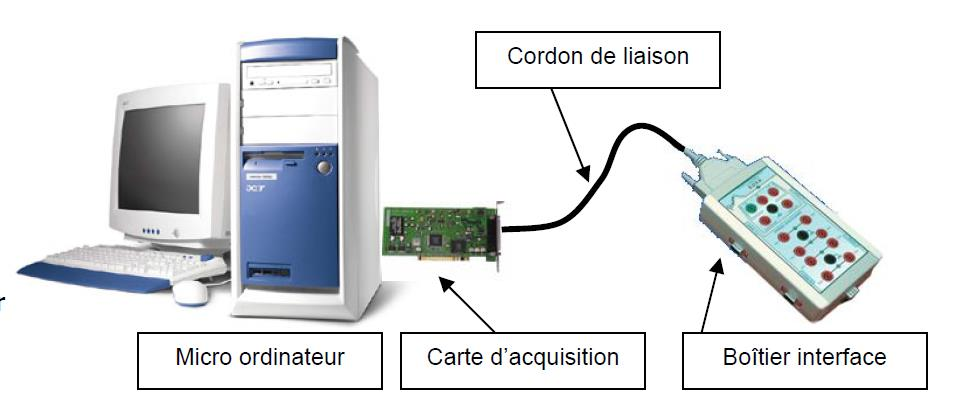
\includegraphics[]{MPI - Physique/TP/tpfig/imgtp4.jpg}}
    
    \begin{experience}{}{}
        Pendant toute la durée du TP, on observera simultanément avec le signal numérique acquis, le signal analogique à l'oscilloscope :
        %
        \begin{enumerate}
            \ithand \hg{Brancher en sortie du GBF} d'une part \hg{la \texttt{voie 1} de l'oscilloscope} mais aussi \hg{l'entrée \texttt{EA0} du boîtier \texttt{SYSAM}} \emph{(sans oublier de brancher aussi la masse)}.
            
            \ithand Une fois \hg{le logiciel \textun{Synchronie} ouvert} l'acquisition se fait dans le bonjour rémi  \hg{menu \texttt{Exécuter}} (ou directement au clavier avec la touche \texttt{F10}). \hg{Vérifier dans le menu \texttt{Paramètre -> Entrées} que l'entrée \texttt{EA0} a bien été sélectionné} .
            
            \ithand \hg{Vérifier que vous obtenez} \emph{\large\EBGaramond a priori} le \hg{même signal à l'oscilloscope et sur \textun{Synchronie}}.
        \end{enumerate}
    \end{experience}
    
    
    
\end{document}